%!TEX TS-program = xelatex
%!TEX encoding = UTF-8 Unicode
% !TEX root = ../../metm.tex

\chapter{STEREOFONIA}
\startcontents[chapters]
\printcontents[chapters]{}{1}{}

\vfill\null

Il primo passo necessario verso la comprensione del concetto di \emph{Stereofonia},
prima di arrivare alle tecniche ed alle tecnologie elettroacustiche che la
rendono possibile, è stabilire attraverso l'etimologia del termine, e dei
termini ad esso collegati, una base concettuale solida. \emph{Stereo}, dal greco
\emph{Stere\'os}, significa \emph{solido}. Non un numero, non una configurazione
ma un aggettivo qualitativo. Nel dizionario inglese Oxford: \emph{Solid, firm
and stable in shape. Having three dimensions}. Solido, \emph{solid}, dalla radice
latina di \emph{Solidus, Sollus}, intero.

Con la parola \emph{Stereofonia} dovremmo quindi descrivere una condizione
nella quale \emph{phon\={e}}, sempre dal greco, \emph{suono}, la \emph{voce},
arrivi all'ascoltatore solida, integra, ferma e stabile nella sua forma (sonora)
multi dimensionale, intera.

%\clearpage

Indispensabile alla comprensione del mondo sonoro elettracustico nelle sue
radici è anche la descrizione del concetto di \emph{mono}, nomignolo di
\emph{monofonico}, espresso nel legame tra \emph{monos} e \emph{phon\={e}}: una voce,
\emph{one voice}, \emph{alone}, sola. La stessa parola usata nella descrizione
del canto gregoriano ad una voce, successivamente evolutasi nella \emph{polifonia}
(dal greco \emph{poluph\={o}nia}, da \emph{polu}, molte e \emph{phon\={e}},
voci). Quindi la dicotomia, se proprio deve essercene una, tra monofonia e
stereofonia semplicemente non esiste. L'estensione del concetto di monofonia,
nel suo eventuale opposto, è polifonia. La stereofonia è semplicemente un
concetto altro.

Con la parola stereofonia dovremmo descrivere anche la condizione in base alla
quale il suono arrivi \emph{solido} all'ascoltatore, \emph{intero, fermo e
stabile} nella sua forma sonora multidimensionale originaria, attraverso
la riproduzione elettroacustica, attraverso la trasmissione e la diffusione mediante
altoparlanti, con un numero qualsiasi, o necessario, di canali. In questo caso,
facendo riferimento alla definizione dell'aggettivo \emph{stereofònico}, ci
si apre alle tecniche ed alle tecnologie che hanno reso possibile la
trasmissione, la riproduzione e la diffusione del suono in stereofonia.
Un aggettivo, \emph{Stereofònico}, che dovrebbe essere usato con cautela, nella
descrizione di tecniche e tecnologie atte alla riproduzione dei suoni in modo
che l’ascoltatore abbia l’impressione di trovarsi nello spazio sonoro originale o,
nel caso non ve ne sia, per sorgenti di natura non acustica, che restituiscano
informazioni tali da descrivere una correlazione al sistema percettivo.

Condizioni di ascolto, dal latino \emph{auscultare}, prestare attenzione a
qualcosa in quanto oggetto o motivo di informazione.%, con specifiche
%caratteristiche di solidità spaziale, dimensionalità osservabili nella forma
%sonora riconoscibile, informativa.

\vfill\null

%------------------------- APPROFONDIMENTO
%\begin{figure}[th]
\begin{tabular}{L{.969\textwidth}}%
\toprule
	\textbf{Alan Dower Blumlein}\\
\midrule
Nato il 29 giugno 1903 a Londra, Deceduto il 7 giugno 1942 a Herefordshire,
Inghilterra, fu ingegnere elettronico presso EMI, per la quale pubblicò brevetti
per le sue numerose invenzioni nel campo delle telecomunicazioni soprattutto in
relazione alle tecnologie di registrazione, trasmissione e diffusione del suono.
Ottiene, nella sua breve carriera, 128 brevetti, motivo per cui è considerato
uno dei più importanti ingegneri e inventori del suo tempo. Morì durante la
seconda guerra mondiale all'età di 38 anni, durante un test militare segreto del
sistema radar H2S allora in fase di sviluppo, a bordo del bombardiere Halifax
su cui stava volando. Tra le numerose invenzioni legate al nome di Blumlein
quelle legate alla Stereofonia stravolsero completamente il mondo della
fruizione pubblica del suono. Le sue prime note sull'argomento risalgono al 25
settembre 1931 e il suo brevetto aveva il titolo “Miglioramenti ai, ed in
relazione ai, sistemi di trasmissione, registrazione e riproduzione del suono”.
La domanda di brevetto fu del 14 dicembre 1931 ed la concessione fu dell
14 giugno 1933, brevetto britannico numero 394.325.\\
\bottomrule
\end{tabular}
%\end{figure}
%------------------------- APPROFONDIMENTO

%%%%%%%%%%%%%%%%%%%%%%%%%%%%%%%%%%%%%%%%%%%%%%%%%%%%%%%%%%%%%%%%%%%%%% LE RADICI
%%%%%%%%%%%%%%%%%%%%%%%%%%%%%%%%%%%%%%%%%%%%%%%%%%%%%%%%%%%%%%%%%%%%%%%%%%%%%%%%
\section{Radici}

L'idea di riprodurre con il suono anche lo spazio che lo caratterizza risale,
come altre idee ed invenzioni legate al mondo della diffusione e riproduzione
dei suoni, alla fine dell'ottocento, nell'era elettrica della rivoluzione
industriale. In quei decenni si svolgevano grandi eventi e mostre di divulgazione
industriale e tecnologica,
come l'\emph{International Exposition of Electricity} tenutasi nel 1881.
Insieme a bulbi luminosi, incandescenze e batterie per l'accumulazione
dell'energia, in quel periodo ci fu spazio anche per l'idea di \emph{telefono stereo},
alla base del \emph{Théâtrophone} di Clément Ader.

Per tutta la durata dell'esposizione, ogni sera nelle sale del \emph{Grande Opera}
di Parigi, veniva suonata musica che il pubblico dell'esposizione poteva ascoltare,
per alcuni minuti, al telefono, a circa due chilometri di distanza presso
il \emph{Palais de Industrie}.

\begin{quote}
One of the most popular attractions at the \emph{Paris Electrical Exhibition} is
the nightly demonstration of the marvelous powers of the Ader telephone, by its
transmission of the singing on the stage and the music in the orchestra of the
\emph{Grand Opera} at Paris, to a suite of four rooms reserved for the purpose
in one of the galleries of the \emph{Palais de l'Industrie}. [\ldots] Certainly
nothing has ever been done before so effectually to popularize science, and to
render the masses familiar with the effect, however ignorant they may be of the
cause, of this marvelous invention, the first feeble voice of which was heard in
the \emph{Centennial Exhibition of 1876}\footnote{ \emph{Scientific American},
December 31, 1881, pages 422-423,\\ \url{https://earlyradiohistory.us/1881opr.htm}\\
Una delle attrazioni più popolari al \emph{Paris Electrical Exhibition} è la
dimostrazione notturna delle meravigliose possibilità del telefono di Ader,
che trasmette dal palco le voci e la musica dell'orchestra del \emph{Grand Opera}
di Parigi ad un gruppo di quattro sale riservate allo scopo in una delle gallerie
del \emph{Palais de l'Industrie}. [\ldots] Certamente nulla è mai stato fatto
prima in modo così efficace per divulgare la scienza e portare le masse a contatto
con l'effetto, per quanto ignoranti possano essere della causa, di questa
meravigliosa invenzione, la cui prima debole voce è stata ascoltata nella
\emph{Mostra del Centenario del 1876}.}.
\end{quote}

\begin{figure}[t]
\centering
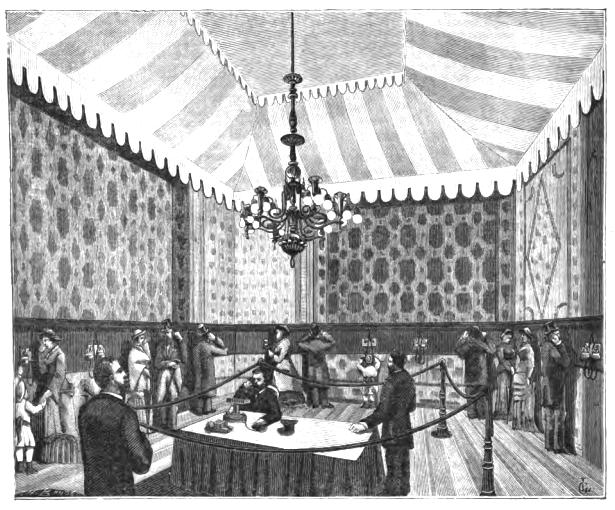
\includegraphics[width=1\columnwidth]{CAPITOLI/1000/IMG/1881opr4.jpg}
\caption{Illustrazione della sala d'ascolto del telefono all'Esposizione di
Parigi del 1881. Gli ascoltatori avevano i ricevitori telefonici per entrambe
le orecchie per ascoltare il programma teatrale in stereo.}
\label{fig:teatrophone2}
\end{figure}

Nonostante il telefono fosse un'invenzione giovanissima, al punto da pensare che
la diffusione del suono dal teatro alla sala d'ascolto avrebbe rappresentato
motivo di interesse da parte del pubblico a prescindere dalla condizionen di
ascolto, Ader aggiunse l'idea di esperienza che, attraverso i concetti di
binauralità e stereofonia, ebbe un impatto incredibile sul pubblico. L'articolo
comparso su \emph{L'Electricien} in cui si descrive il funzionamento
dell'invenzione fu firmato da M. Hospitaller che descrive così l'esperienza di
ascolto:

\begin{figure}[t]
\centering
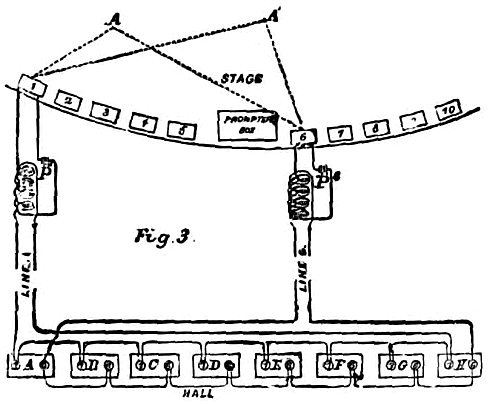
\includegraphics[width=1\columnwidth]{CAPITOLI/1000/IMG/1881opr2.jpg}
\caption{Disposizione dei trasduttori sul palco e collegamento alle due linee
telefoniche. Ogni ascoltatore è posizionata di fronte ad una coppia di telefoni
i quali ricevono il segnale da due trasduttori distinti posizionati sul palco.
Questi trasduttori sono raggruppati in coppie forniscono segnale a sedici
telefoni, accoppiati per otto ascoltatori.}
\label{fig:teatrophone1}
\end{figure}

\begin{quote}
We will now consider the new acoustic effect which Mr. Ader has discovered, and
applied for the first time in the telephonic transmission at the Electrical
Exhibition. Every one who has been fortunate enough to hear the telephones at
the Palais de l'Industrie has remarked that, in listening with both ears at the
two telephones, the sound takes a special character of relief and localization
which a single receiver cannot produce. [\ldots] As soon as the experiment
commences the singers place themselves, in the mind of the listener, at a fixed
distance, some to the right and others to the left. It is easy to follow their
movements, and to indicate exactly, each time that they change their position,
the imaginary distance at which they appear to be. [\ldots] This phenomenon is
very curious, it approximates to the theory of binauriclar auduition, and has
never been applied, we believe, before to produce this remarkable illusion to
which may almost be given the name of auditive perspective. [\ldots] In order
to realize it, we may recall the stereoscope, which allows us to see objects in
their natural relief\footnote{
\emph{Scientific American}, December 31, 1881, pages 422-423,\\
\url{https://earlyradiohistory.us/1881opr.htm} \\
Considereremo ora il nuovo effetto acustico che il signor Ader ha scoperto e
applicato per la prima volta nella trasmissione telefonica all'esposizione
elettrica. Tutti coloro che hanno avuto la fortuna di ascoltare i telefoni al
\emph{Palais de l'Industrie} hanno osservato che, ascoltando con entrambe le
orecchie ai due telefoni, il suono assume un carattere speciale di meraviglia e
localizzazione, cosa che un singolo ricevitore non può produrre. [\ldots] Non
appena inizia l'esperimento, i cantanti si posizionano, nella mente
dell'ascoltatore, a una distanza fissa, alcuni a destra e altri a sinistra. È
facile seguire i loro movimenti e indicare esattamente, ogni volta che cambiano
posizione, la distanza immaginaria alla quale sembrano essere. [\ldots] Questo
fenomeno è molto curioso, si avvicina alla teoria dell'audizione biauricolare che
crediamo non sia mai stato applicato prima di produrre questa straordinaria
illusione, a cui potrebbe essere dato il nome di prospettiva auditiva. [\ldots]
Per realizzarlo, possiamo ricordare lo stereoscopio, che ci consente di vedere
gli oggetti nel loro rilievo naturale.}.
\end{quote}

Tra le varie definizioni di stereofonia il termine è inoltre usato per indicare
la parte dell’acustica fisiologica che si occupa del fenomeno dell'ascolto
biauricolare del sistema uditivo. Tale fenomeno conferisce alla percezione umana
il potere localizzatore, cioè la capacità, dovuta al lavoro congiunto dei due
sistemi auricolari separati ed al sistema nervoso centrale, di determinare la
direzione di provenienza di un suono. In tal senso, esiste in acustica
fisiologica la definizione di monofonia in qualità di condizione anomala del
sistema percettivo, caratterizzata dalla mancanza degli elementi necessari a
individuare i caratteri spaziali dei suoni stessi, come per esempio quella
ottenuta con un solo orecchio.

La percezione dei caratteri spazio-temporali dei suoni, in particolare della
loro direzione di provenienza e della loro relazione con lo spazio che
attraversano, definiscono i tratti essenziali della stereofonia, in relazione
all'udito, in virtù dell’audizione biauricolare (o binaurale).

\begin{quote}
When recording music considerable trouble is experienced with the unpleasant
effects produced by echoes wich in the normal way would not be noticed by anyone
listening in the room in which the performance is taking place.
An observer in the room is listening with two ears, so that echoes reach him
with the directional significance which he associates with the music performed
in such room. He therefore discount these echoes and psychologically focuses
his attention on the source of the sound. When the music is reproduced through
a single channel the echoes arrive from the same direction as the direct sound
so that confusion results. [\ldots] Human ability to determine the direction
from which sound arrives is due to binaural hearing, the brain being able to
detect differences between sound received by the two ears from the same source
and thus to determine angular directions from which various sounds
arrive\footnote{[\cite{ab58}] - Quando si registra musica acustica, si riscontrano
notevoli problemi a causa degli effetti indesiderati prodotti dalle riflessioni
acustiche dell'ambiente, che nell'ascolto normale non vengono notati dagli
ascoltatori nella stanza in cui si svolge l'esibizione.
Un osservatore nella stanza sta ascoltando con due orecchie, in
modo che gli echi lo raggiungano con il significato direzionale che associa alla
musica eseguita in quella stanza. Pertanto, non tiene conto di questi echi e
focalizza psicologicamente la sua attenzione sulla fonte del suono. Quando la
musica viene riprodotta attraverso un singolo canale, gli echi arrivano dalla
stessa direzione del suono diretto, in modo da creare confusione. [...] La
capacità umana di determinare la direzione da cui proviene il suono è dovuta
all'udito binaurale, il cervello è in grado di rilevare le differenze tra il
suono ricevuto dalle due orecchie dalla stessa fonte e quindi di determinare le
direzioni angolari da cui provengono i vari suoni.}.
\end{quote}

È con queste parole che Blumlein nel 1931 descriveva i fondamenti delle conoscenze
in termini di percezione dei suoni e di come questi venivano utilizzati per definire
criteri tecnologici adeguati per la riproduzione dei suni. Ed è per questo che
in maniera piuttosto discreta intitola testo del brevetto che ha dato la nascita
commerciale e tecnologica alla stereofonia \emph{Miglioramenti in, ed in relazione,
ai sistemi di trasmissione del suono, registrazione del suono e riproduzione del suono}.
Genrico, inglese, la binauralità dell'ascolto umano è la prima affermazione di
Blumlein: “\emph{un osservatore nella stanza sta ascoltando con due orecchie}”.
Come questa condizione di ascolto si evolva nel tempo è la peculiarità della
stereofonia.

Il documento presenta diverse tecniche stereofoniche di microfonazione, di
incisione del disco e di trasmissione radio. La domanda fu presentata nel
dicembre 1931 ed approvata nel giugno 1933. Nel testo fa riferimento al cinema,
consapevole della necessità di migliorare la resa della registrazione sonora
in situazioni di “realismo”.

\emph{Una voce in una piccola stanza riverberante è una condizione d'ascolto che
rispetti qualità di stereofonia?}

In funzione di dei riferimenti storici e delle descrizioni fatte finora, la
risposta è chiaramente affermativa. Anche con un solo oggetto sonoro, una sola
voce, in una piccola stanza, siamo in presenza di un fenomeno acustico
stereofonico, percepito bianuralmente. Su questa condizione Blumlein presenta
le basi teoriche e tecnologiche della stereofonia, nel brevetto in cui ne
rende i concetti fondamentali, solidi, stabili nel tempo e nello spazio delle
parole.


%%%%%%%%%%%%%%%%%%%%%%%%%%%%%%%%%%%%%%%%%%%%%%%%%%%%%%%%%%%%%%%%%%% SECTION FOUR
%%%%%%%%%%%%%%%%%%%%%%%%%%%%%%%%%%%%%%%%%%%%%%%%%%%%%%%%%%%%%%%%%%%%%%%%%%%%%%%%
\section{Ramificazioni}

Con la profonda conoscenza del significato del tempo tra noi e Blumlein,
possiamo esporre il significato degli altoparlanti meglio di lui. Per l'era
Blumlein, l'altoparlante era lo strumento futuro per un tempo presente migliore.
Il suono riprodotto, alla sua giovane età, era pura magia. Oggi sappiamo bene
quanto siamo insoddisfatti della riproduzione degli altoparlanti. Quando il
primo iPhone è stata l'unica cosa intelligente sul pianeta, è stato fantastico,
un fantastico oggetto di creazione. Oggi con lo stesso oggetto non faremmo
nemmeno una foto. Ascoltare un assolo di violino riprodotto dal miglior
altoparlante sul mercato non è la stessa esperienza della performance reale.
Non è legato alla stereofonia e all'abilità tecnica, è parte integrante del
limite di riproduzione della tecnologia che siamo in grado di realizzare.
%
Sostituendo la voce umana che parla dell'esempio precedente, con un singolo
altoparlante che parla delle registrazioni di quella voce umana perdiamo, come
descritto da Blumlein, la capacità delle orecchie-cervello decifra la relazione
suono-ambiente. Non è più lo stesso ascolto stereofonico. Il numero di fonti è
lo stesso. Entrambi nel loro linguaggio monofonico producono una diversa
condizione di ascolto.%

Nel 1992 Michael Gerzon \cite{mg92pdmsss} disegna una rappresentazione
schematica delle diverse posizioni degli altoparlanti per stereo multispeaker,
da una a cinque:

\begin{quotation}
\ldots we show the loudspeaker layouts considered for frontal stage stereo
using from one (regarding mono as the trivial case of “one-loudspeaker stereo”!)
to five loudspeakers…
\end{quotation}

Esiste una condizione stereo con un solo altoparlante? Davvero si.

Un altoparlante in grado di suonare se stesso, non riproducendo qualcosa di
reale acustico ma producendo un suono che non potrebbe vivere senza un
altoparlante, rappresenta una condizione stereo con caratteristiche generali
simili alla voce parlante. Un rumore rosa filtrato da Butterworth che canta
monofonicamente in una stanza è una condizione di stereofonia.

Per un musicista elettroacustico, gli altoparlanti sono strumenti. La scelta
degli altoparlanti, la conoscenza del loro carattere e delle loro
caratteristiche è un momento necessario per quel musicista. Conoscere il loro
personaggio richiede tempo. Cambiare manualmente la frequenza di un suono
sinusoidale riprodotto da un altoparlante a tre vie, a un metro di distanza,
con le orecchie alla stessa altezza del centro dell'altoparlante, è un buon modo
per dire Ciao! all'altoparlante. Il musicista scoprirà in questo modo che i
suoni prodotti dall'altoparlante cambieranno forma durante lo spazzamento. Forse
vicino al punto di incrocio del crossover troverà alcune peculiarità, altre
strane decorrelazioni di fase ad altissima frequenza. Gli altoparlanti sono
strumenti. Due altoparlanti potrebbero essere il minimo impostato per la
condizione stereofonica di ascolto. Potrebbero essere cantanti elettroacustici
polifonici. Potrebbero anche essere una condizione monofonica, quando non sono
richieste stereofonia o polifonia.%

\begin{figure}[h]
\begin{center}
  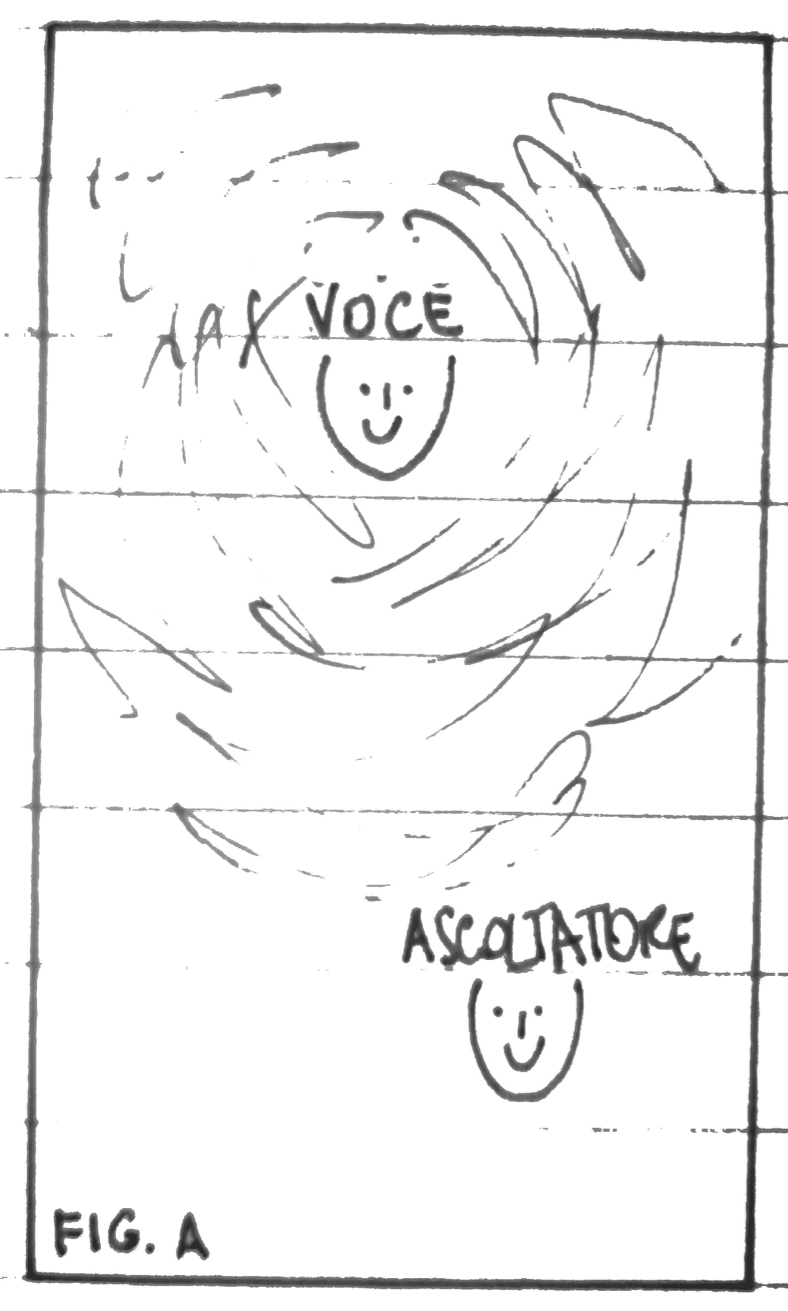
\includegraphics[width=.48\linewidth]{CAPITOLI/1000/IMG/figa.png}
%\caption{}
\label{ee:figa}
\end{center}
\end{figure}

Una voce nello spazio di una stanzetta si dirige, con una sua direzione, verso
un punto e contemporaneamente, con meno direzionalità, lateralemente, raggiunge
il resto della stanza. Questo meccanismo ha a che fare con la forma sonora di una
voce, prima ancora che con la forma architettonica della piccola stanza.

Dobbiamo immaginare la forma sonora come un'armatura attorno al nostro oggetto
sonoro, un'armatura fatta di fittissime molecole in vibrazione. Ogni suono ha una
sua veste plastica. Se vi dicessi ottavino e poi contrabbasso voi avreste già
collegato tutto ciò che vi serve per vederli, sentirli, ed ora, volendo, vestirli
della loro forma sonora. Ma cosa accade alla forma sonora di uno strumento in
presenza di tecninche estese applicate allo strumento? Una mano che inizia a produrre
suono li, nello stesso luogo dello strumento, a dove pochi minuti prima premeva
solo tasti (la mano  sinistra di UR) diventa esplosione di forma acustica e musicale.

Ecco questo è un po' il cuore di quello che vorrei fosse il mio dottorato di
ricerca che non avrò mai e un po' anche la manifestazionne di una piuttosto
triste verità: esclusi i percorsi individuali e rari percorsi di ricerca
non istituzionalizzata, la musica contemporanea ha esaurito la sua carica
contributiva al conoscimento, alla comprensione generalizzata.

Tornando alla forma, Questa si staglia nello spazio circostante e si espande e si muove
all'interno di questo spazio e ne viene modellata come una massa morbida all'interno
di un contenitore. Qui iniziano i fenomeni di riflessione e la forma si
cristallizza assumendo caratteristiche in funzione dello spazio e, quindi, del tempo.
L'ascoltatore che partecipa a questo evento vede una persona solida parlare nello
spazio di una stanza e sente la forma solida della voce provenire dalla sua bocca
e contemporaneamente, quindi subito dopo, dalla stanza sotto forma di riflessioni.
Sì! converremo infine, questa esperienza di ascolto rispetta queste qualità.

\begin{figure}[h]
\begin{center}
  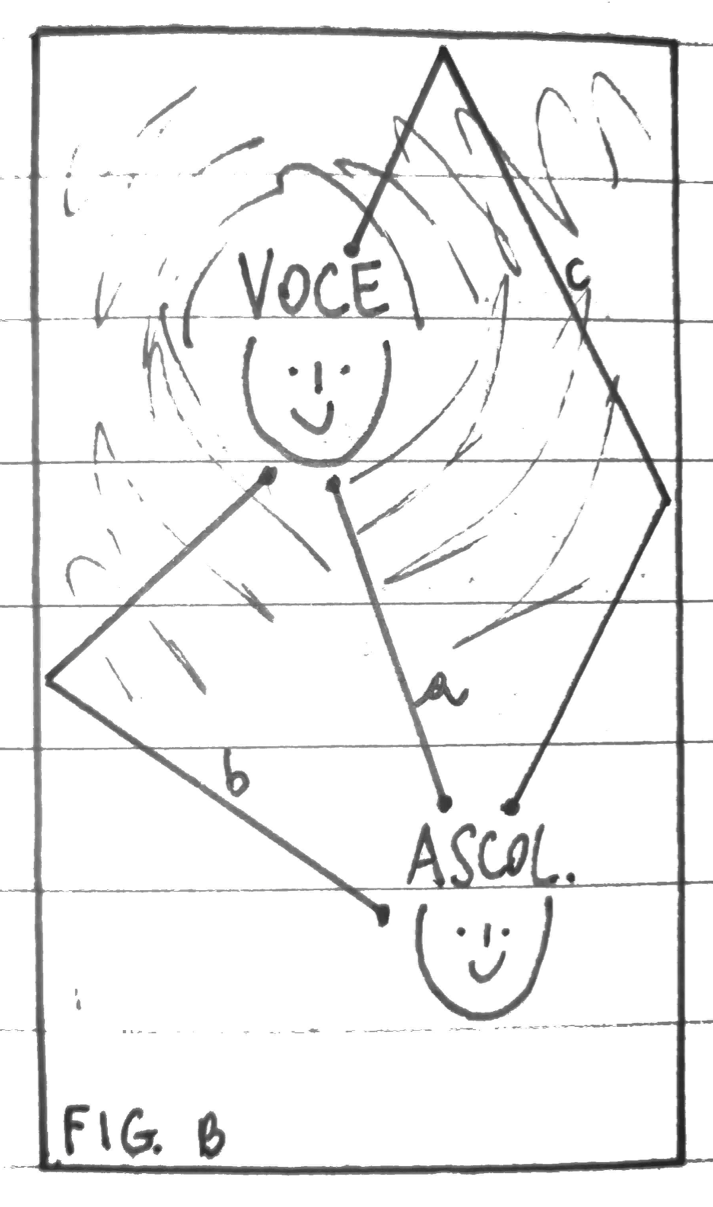
\includegraphics[width=.48\linewidth]{CAPITOLI/1000/IMG/figb.png}
%\caption{}
\label{ee:figb}
\end{center}
\end{figure}

Una voce che attraverso la sua forma acustica riempia uno spazio acustico è
un'esperienza d'ascolto stereofonica. Non è ancora giunto il momento di
interrompere la discussione dicendo: “ma come, non servono due diffusori?” Non
ancora, il problema è più complesso. È importante sottolineare che la stereofonia,
l'ascolto stereofonico, è una qualità dell'ascolto che si può osservare in
determinate circostanze e che richiede necessariamente il lavoro concertato delle
due orecchie. Un ascolto stereofonico è quindi possibile solo in coincidenza
con un ascolto \emph{binaurale}, ovvero effettuato con entrambe le orecchie.

Di nuovo una qualità che presuppone dei contenuti coerenti con delle
caratteristiche specifiche. Ora, nel mondo elettroacustico, del suono prodotto
o riprodotto elettricamente, dovremmo essere in grado di effettuare lo stesso
ragionamento sostituendo alla persona che parla un diffusore generico. Come per
l'essere umano, la voce è esempio di suono proprietario anche per il diffusore
si può scegliere un suono che lo caratterizzi elettroacusticamente, un suono
che lo rende particolare: il suono definito rumore rosa. Posizionato il diffusore
nella stessa stanza e con le stesse circostanze di ascolto precedenti, avremmo
una condizione di ascolto stereofonico? Ovviamente si. Un solo diffusore può
costituire una condizione d'ascolto stereofonica. In questo caso l'oggetto
acustico è un diffusore che esprime se stesso attraverso un suono non informativo.
Un rumore è caratterizzato da un'assenza di informazione, fatta esclusione del
fatto stesso che è rumore.

\begin{figure}[h]
\begin{center}
  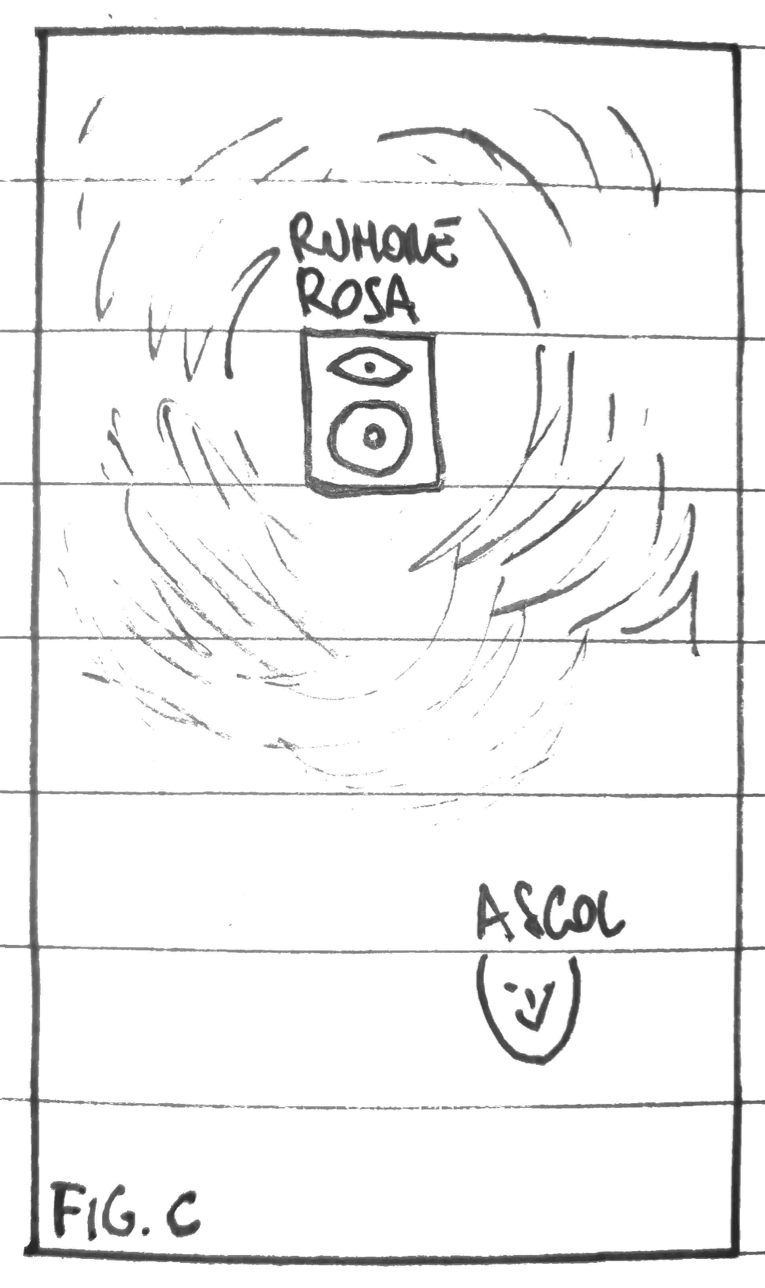
\includegraphics[width=.48\linewidth]{CAPITOLI/1000/IMG/figc.png}
%\caption{}
\label{ee:figc}
\end{center}
\end{figure}

che informazioni? be quelle che descrivono un suono come la percezione di altezza,
durata, intensità e timbro. Questa descirizione di stereofonia possibile anche
con un solo soggetto sonoro, voce o diffusore che sia, non è così comune e
condivisa. Ciò accade a causa del fatto che spesso si fa confusione tra stereofonia,
o stereofonica, come aggettivo applicato alla tecnica di diffusione e registrazione
piuttosto che alla qualità percettiva che queste tecniche dovrebbero suggerire.

Per arrivare a descrivere la tecnica dobbiamo percorrere ancora alcuni passi.

Nel momento in cui si passa da un dominio puramente acustico sia esso derivante
da una voce umana quanto un rumore diffuso attraverso un altoparlante, ad un
dominio di riproduzione acustica, ovvero di rappresentazione attraverso meccanismi
e tecniche allora cambia completamente lo scenario acustico e le circostanze di
ascolto. Un diffusore tradizionale può riprodurre una voce umana o un diffusore
che suona rumore rosa? Si certo che può riprodurli. Questa riproduzione
costituirebbe un ascolto stereofonico della sorgente originale? No, non lo sarebbe.

\begin{figure}[h]
\begin{center}
  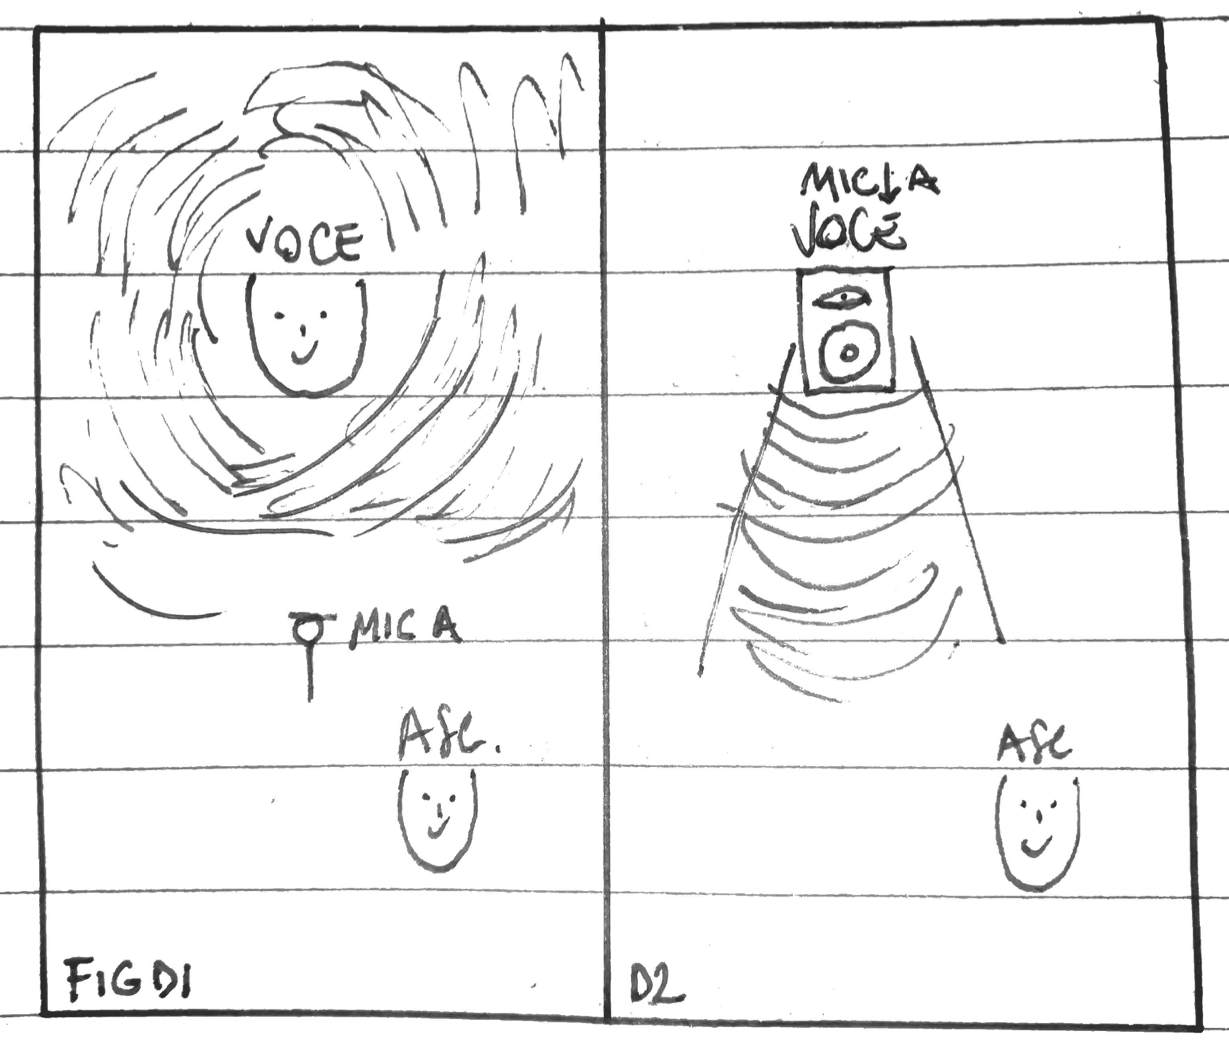
\includegraphics[width=.98\linewidth]{CAPITOLI/1000/IMG/figd1d2.png}
%\caption{}
\label{ee:figd1d2}
\end{center}
\end{figure}


\begin{quote}
When the music is reproduced through a single channel the echoes arrive from the same direction as the direct sound so that confusion result\footnote{Quando la musica viene riprodotta attraverso un singolo canale, gli echi arrivano dalla stessa direzione del suono diretto in modo tale da creare confusione.}.
\end{quote}

Qui si sviluppa tutta la questione, un solo diffusore non è in grado di rappresentare
la solidità originaria, la forma sonora dell'oggetto acustico originario, il suo
rapporto con lo spazio che lo ha modellato. Per comprendere meglio ogni possibile
questione legata alla diffusione sonora, mediante dispositivi elettroacustici ci
vorrebbe un minimo di tempo speso nella sperimentazione con lo strumento altoparlante.
Perché di questo si parla, di uno strumento tecnico, tecnologico, musicale e
profesisonale.

\begin{quote}
Ci sono problemi che alle volte anch'io non capisco, nel senso che se ne porgono
continuamnte di nuovi. È da anni che lavoro e sperimento negli studi di live electronics di
Friburgo, della Sudwestfunk. Si tratta delle trasformazioni in tempo reale del
suono e della voce, e del comporla con lo spazio, usando le tecnologie di oggi,
con i vari altoparlanti disposti nella sala. C'è qualcosa di nuovo solo sul piano
tecnico, perché  se prendiamo la Scuola di S. Marco veneziana di Andrea e Giovanni
Gabrieli, Monteverdi, di Willaert, con le composizioni a più cori, la grande
scuola spagnola all'epoca di Filippo II [\ldots] si faceva musica per otto organi
e quattro cori, cioè si suonava lo spazio come componente musicale, non come poi
la prassi dell'ottocento usa lo spazio, mettendo dentro l'orchestra e quel che
succede succede. Quindi altri studi, anche studi di fisica architettonica, studi
di processi di eco, di riverberazione, di materiali acustici. [\ldots] Qui una
composizione non è  data una volta per sempre, perché per ogni spazio noi dobbiamo
cambiare i programmi dei computer e modificando i rapporti della trasformazione si modifica anche il rapporto acustico; [\ldots] il grande fascino di questo per me
è veramente la non ripetitività. [\ldots] Un interprete non deve studiarsi la
parte ma veramente partecipare. [\ldots] Cioè vedi come noi possiamo con la
tecnologia di oggi studiare molto meglio, cioè studiare in un altro modo. \\
Luigi Nono 1986
\end{quote}

La parabola bacchiana si conclude con una nota autobiografica. Noi, che abbiamo
osservato da vicino la maledizione di Bacco, non possiamo più tacere e seminiamo,
il vento muoverà le orecchie penzolanti e porterà le nostre confessioni altrove.
%%%%%%%%%%%%%%%%%%%%%%%%%%%%%%%%%%%%%%%%%%%%%%%%%%%%%%%%%%%%%%%%%%%%%%%%%%%%%%%%%%%%%%%%%%%%%%%%%% fiune dalle esposizioni

Una singola voce umana, monofonica, sta parlando all'interno di una piccola
stanza, una condizione stereofonica accettabile? In accordo con Blumlein,
Sì! Questo è il primo punto fermo.

Michael Gerzon, dagli anni settanta agli anni novanta, dalle radici dell'era di
Blumlein ha saltato la linea con una dozzina di descrizioni chiare sulla
percezione e tentativi di progettare tecnologie di riproduzione per colmare il
divario rispetto al regno acustico.

\begin{quotation}
The ears and brain localize sounds according to many different mechanism. Among
the most important cues used are low frequency interaural phase (applicable up
to around 2\emph{KHz}, but dominant below 700\emph{Hz}) and localization by
amplitude differences between the two ears, predominantly above about
1\emph{KHz}. While other cues are also important, we have found that satisfying
both these cues, and making them mutually consistent for central listener facing
in any direction, leads to particularly robust and reliable localization
quality.\cite{mg92pdmsss}
\end{quotation}

%%%%%%%%%%%%%%%%%%%%%%%%%%%%%%%%%%%%%%%%%%%%%%%%%%%%%%%%%%%%%%%%%%%% SUBSECTION
%%%%%%%%%%%%%%%%%%%%%%%%%%%%%%%%%%%%%%%%%%%%%%%%%%%%%%%%%%%%%%%%%%%%%%%%%%%%%%%%
\subsection{Sul concetto di \emph{PanPot}}
\label{sec:panpot}

L'oggetto \emph{panner} è rappresentato da un potenziometro di controllo
(hardware o software, in entrambi i casi a controllo analogico o digitale) che
regola la distribuzione di un segnale su più canali componenti un campo sonoro
stereo o multicanale. Ogni mixer ha un \emph{panpot} (abbreviazione di
\emph{potenziometro di panoramica}), per ciascun canale sorgente in ingresso,
che regola l'azione del \emph{panner}.

%L'ultima precisazione riguarda il movimento panoramico. La distribuzione dell'energia
%o la condizione della coppia di segnali che regola il movimento panoramico troppo
%spesso sono descritti come la possibilità di muovere gli oggetti attorno alla posizione
%dell'ascoltatore.

Generalmente il \emph{panpot} viene descritto come un pomello che permette di
muovere i suoni tra la sinistra e la destra del panorama di diffusione, il che è
parzialmente vero e potenzialmente pericoloso in termini di immaginazione
acustica.

Soffermandosi ad analizzare il fenomeno acustico di un suono prodotto da un
oggetto in movimento tra la destra e la sinistra di un campo percettivo emergono
diversi problemi.

Il primo riguarda l'\emph{effetto doppler}. Siamo seduti su una panchina al
margine di una strada che si estende infinita agli estremi della nostra vista
periferica. Un mezzo di soccorso, con la sirena accesa, si avvicina percorrendo
la strada davanti al nostro viso, da sinistra verso destra: percepiamo
una variazione in frequenza al passaggio della sirena, in funzione della
velocità. L'\emph{effetto doppler} ci descrive come nel percorso di
avvicinamento a noi la frequenza sale lentamente fino al massimo ottenuto nel
momento in cui ci raggiunge per poi diminuire rapidamente in coincidenza con
l'allontanamento.

Ora siamo dei \emph{sound designer}, siamo seduti di fronte alla nostra console
analogica e dobbiamo replicare l'effetto sopra descritto. Applicando un
movimento da sinistra a destra, azionando il \emph{panpot} su un suono di sirena
statico, registrato fermo ad un metro di distanza, pur ruotando velocemente il
potenziometro non otteniamo variazioni in frequenza. Il suono si muove tra la
sinistra e la destra del sistema d'ascolto senza produrre il movimento nello
spazio ma solamente lo spostamento della posizione relativa al nostro punto di
ascolto. Ne deriva una prima conslusione: il \emph{panpot} regola una posizione
relativa, non stabilisce criteri di movimento.

Un altro problema emergente del pensare il \emph{panning} come un movimento
scaturisce dalla relazione della sorgente con l'ambiente circostante. Che
movimento può esserci senza tenere conto del luogo in cui la sorgente sonora si
trova? Un avvocato pronuncia la sua arringa in tribunale parlando ad alta voce,
camminando, rimbalzando tra destra e sinistra. La voce si propaga nello spazio
ed è inevitabile che se ne percepisca la variazione topologica, morfologica in
relazione con le caratteristiche architettoniche: a sinistra della stanza c'è
una parete di finestre, a destra un muro in cemento. Pur non avendo velocità
sufficiente ad innescare l'effetto doppler, la sua continua variazione di
posizione corrisponde ad una continua variazione di rapporto con l'ambiente che
lo circonda, in relazione ad ogni infinto punto di ascolto all'interno della
stanza. In altre parole, quel movimento assume significati diversi relativi al
punto di ascolto.

Dovendo simulare lo stesso effetto mediante l'azione sul panpot, otterremmo la
variazione di posizione della voce nello spazio, ma non la sua relazione con lo
spazio.

\begin{figure*}[t!]
    \centering
    \begin{subfigure}[t]{0.45\textwidth}
        \centering
        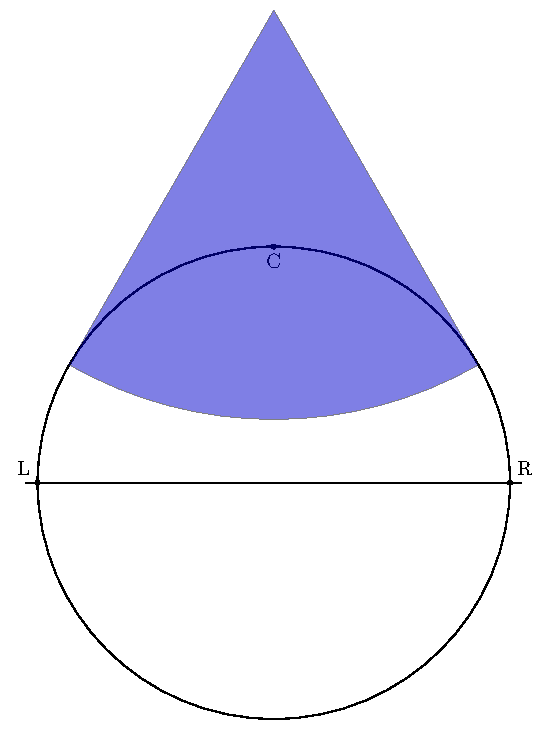
\includegraphics[height=8cm]{CAPITOLI/_TIKZ/PANNING/pan-frontal}
        \caption{Sorgente con incidenza frontale.}
        \label{pan:frontal}
    \end{subfigure}%
    ~
    \begin{subfigure}[t]{0.45\textwidth}
        \centering
        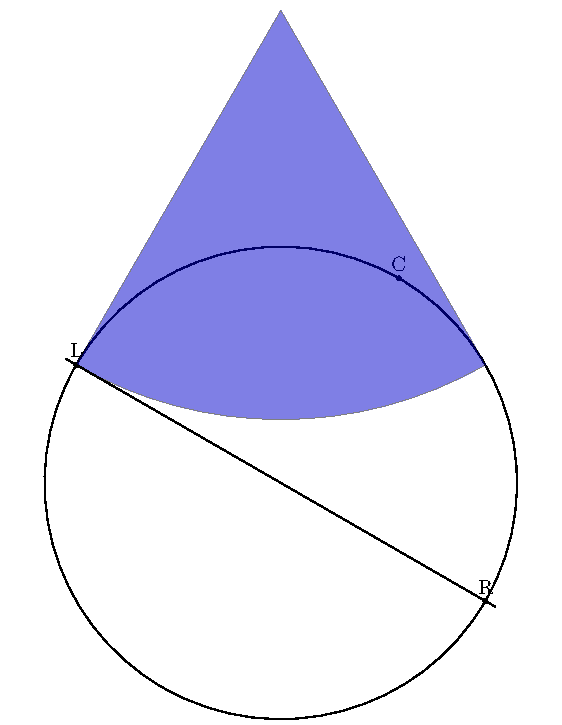
\includegraphics[height=8cm]{CAPITOLI/_TIKZ/PANNING/pan-left}
        \caption{Sorgente con incidenza laterale sinistra di 30 gradi.}
        \label{pan:left}
    \end{subfigure}
    \\
    \begin{subfigure}[t]{0.9\textwidth}
        \centering
        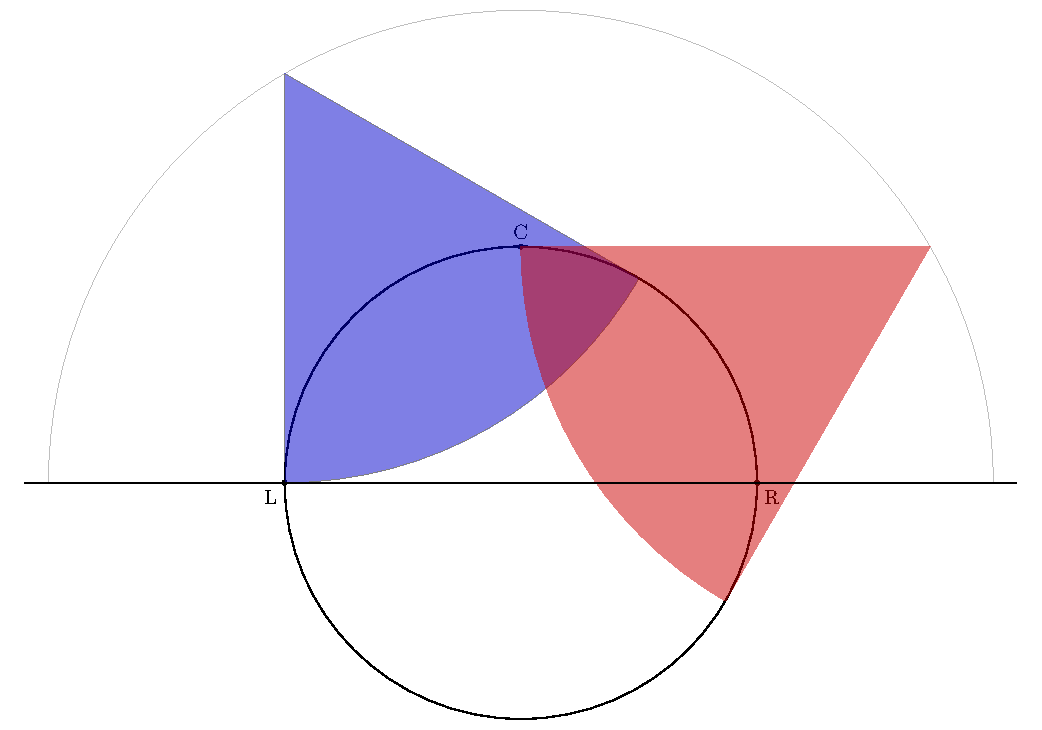
\includegraphics[height=8cm]{CAPITOLI/_TIKZ/PANNING/pan-both}
        \caption{Due sorgenti, una con incidenza laterale sinistra di 30 gradi,
        l'altra con incidenza laterale destra di 60 gradi.}
        \label{pan:both}
    \end{subfigure}
    \caption{La rotazione del \emph{PanPot} esegue una modifica della condizione
    di ascolto dell'ascoltatore, non un movimento della sorgente. Posizionando
    le singole sorgenti ci si pone in ascolto laterale, ruotati. Nella
    sovrapposizione di molteplici sorgenti il panorama risulta composto da
    ognuna di queste, con posizioni assolute ed angoli di incidenza relativi
    della testa.}
    \label{pan:all}
\end{figure*}

Il \emph{panpot}, nella sua capacità di descrizione della relazione tra i canali
che ricevono i suoi segnali, non muove la sorgente nello spazio, ma regola la
posizione della sorgente stessa in relazione al nostro punto di ascolto. In
altri termini il \emph{panner} non regola il movimento della sorgente, ma la
rotazione della testa in relazione ad essa. Il \emph{panner}, muove langolo di
incidenza del suono, ruota la testa, nei confronti della sorgente immobile.

Ogni \emph{panner} ha un'architettura interna che determina la quantità e la
condizione del segnale sorgente per ogni canale di destinazione. I più semplici
suddividono i segnali audio nei due canali sinistro e destro, attraverso un
opportuno controllo di guadagno (volume) discreto. La distribuzione dell'energia
tra i due canali è chiamata legge ed è descrivibile con una funzione matematica.

Come descritto da Blumlein, la sola variazione di ampiezza nella
rappresentazione del panorama stereofonico rappresenta una parte nella complessa
soddisfazione della percezione binaurale, non disegna l'intero meccanismo.
Per questo motivo, prima di descrivere i sistemi di panning di ampiezza, che
sono universalmente implementati su tutti i mixer del pianeta, è più opportuno
riprendere da dove egli stesso è partito. La visione di Blumlein fu ripresa in
seguito da Michael Gerzon, negli anni settanta, per sviluppare la tecnologia
\emph{ambisonic}, la quale rimane un atto di descrizione del mondo sonoro
percepito e riprodotto, nell'evoluzione della stereofonia, completamente diverso
da quello che commercialmente si è diffuso ed imposto.

%%%%%%%%%%%%%%%%%%%%%%%%%%%%%%%%%%%%%%%%%%%%%%%%%%%%%%%%%%%%%%%%%%%% SUBSECTION
%%%%%%%%%%%%%%%%%%%%%%%%%%%%%%%%%%%%%%%%%%%%%%%%%%%%%%%%%%%%%%%%%%%%%%%%%%%%%%%%
\subsection{Sul concetto di \emph{Diagramma Polare}}
\label{sec:polarplot}

Il diagramma polare (o curva polare) è invece un grafico a disegno circolare
dove i parametri sono dati dall’ampiezza e dall’angolo d’incidenza, mentre le
frequenze sono rappresentate da famiglie di curve. In presenza di un’unica curva,
si intende che questa è riferita ad una frequenza di $1KHz$. %piero

Un singolo segnale, nella sua oscillazione, espressa nella variazione di ampiezza
attorno allo zero, potrebbe essere derivato da qualsiasi tipo di microfono senza
un significato particolare. Potrebbe essere generato elettricamente da un
microfono con modello polare particolare o da una fonte sintetica senza
alcuna rilevanza specifica. La provenienza polare, la forma che assume la fase
del segnale, diventa rilevante nel confronto tra segnali.

Il diagramma polare di un microfono che, per caratteristiche costruttive, non
percepisce variazioni di angolo di incidenza del segnale, quindi non-direzionale,
è definito comunemente come omnidirezionale, la sua equazione contiene solo
variazioni di ampiezza, derivate della variazione di pressione dell'aria

\begin{equation}
ndp = 1(x)
\label{eq:omni}
\end{equation}

\begin{figure}[h]
\centering
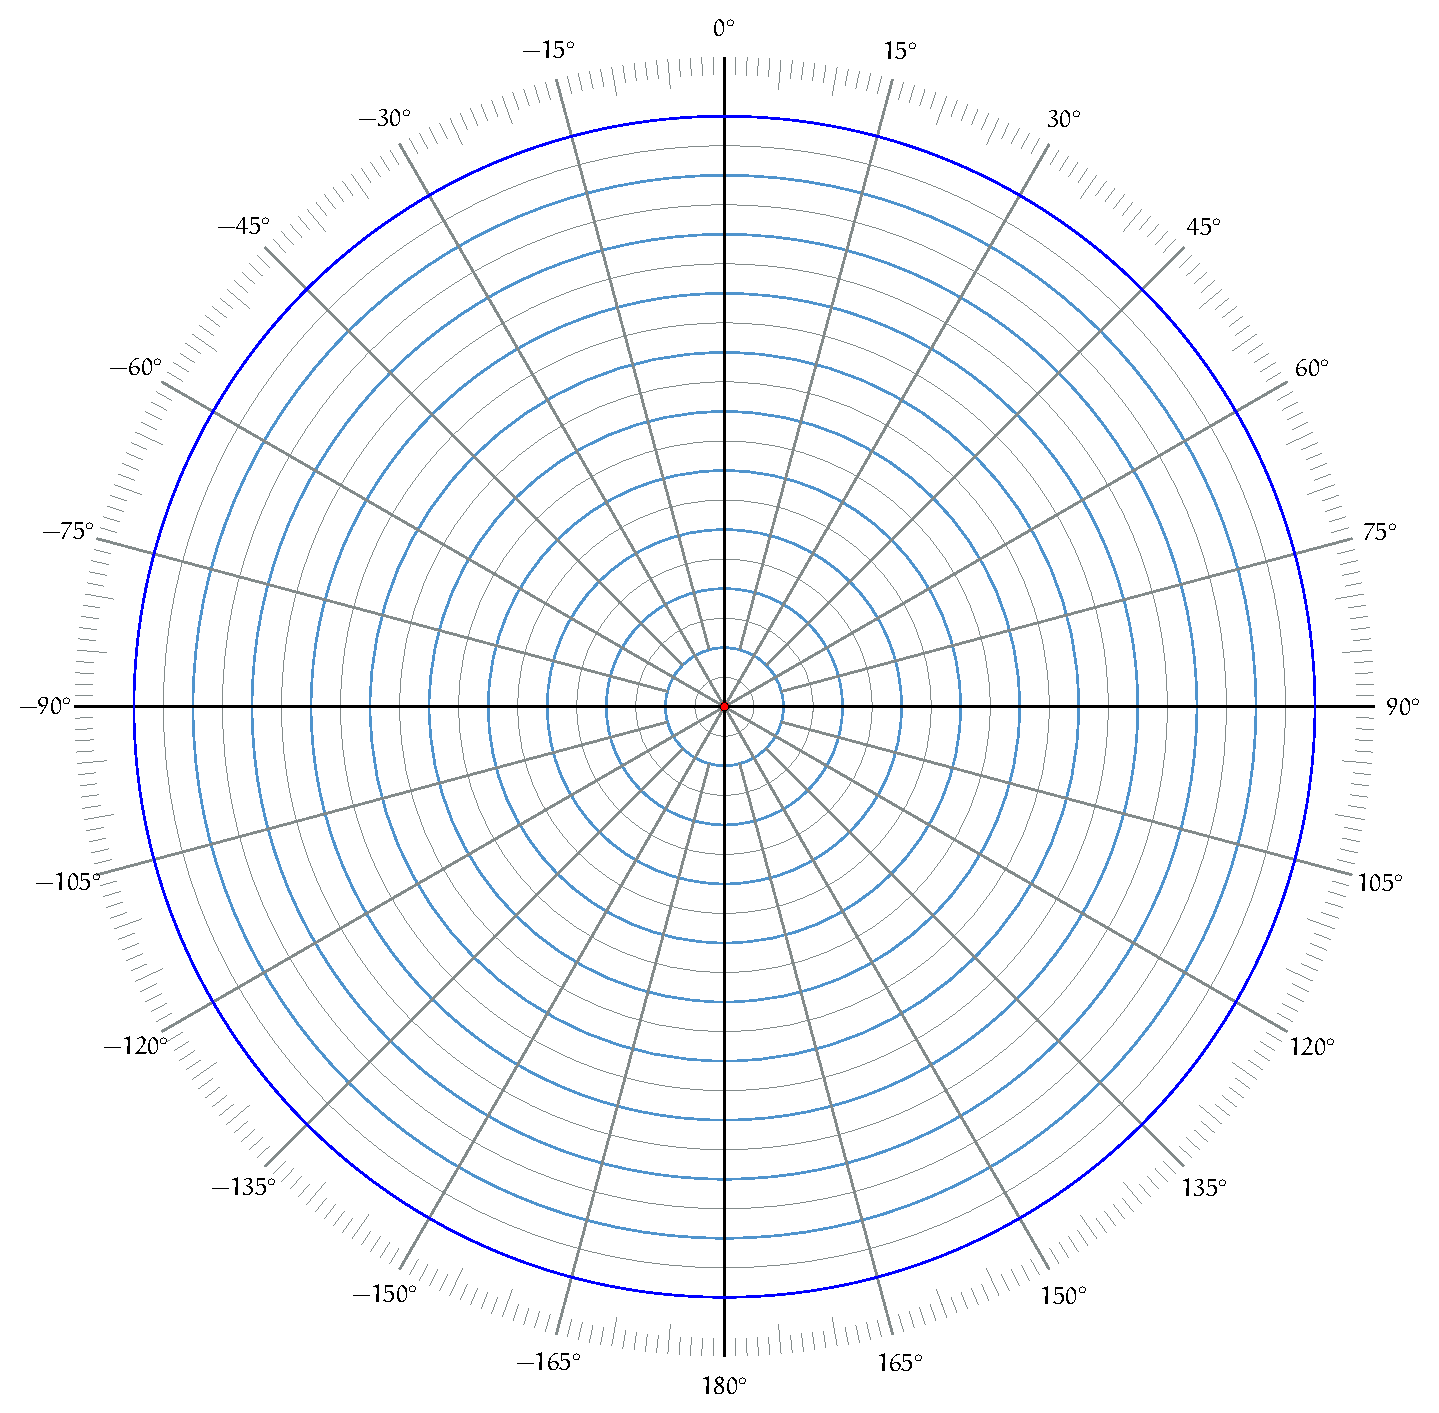
\includegraphics[width=1\columnwidth]{CAPITOLI/_TIKZ/POLAR/omni}
\caption{non-directional}
\label{polar:omni}
\end{figure}

%Il disegno nella parte sinistra di fig. 8 rappresenta la struttura di un tipico microfono a pressione (pressure microphone) omnidirezionale, mentre nella parte destra è rappresentata la sua curva polare, dove vediamo che la direzionalità del suono inizia ad essere percepita dal microfono a partire da circa 5 KHz in su, mentre le frequenze gravi non sono indicate in quanto assimilabili a quella rilevata a 1 KHz, cioè con attenuazione zero per qualsiasi angolo di provenienza del suono.


% %%%%%%%%%%%%%%%%%%%%%%%%%%%%%%%%%%%%%%%%%%%%%%%%%%%%%%%%%%%%%%%%% SECTION FIVE
% %%%%%%%%%%%%%%%%%%%%%%%%%%%%%%%%%%%%%%%%%%%%%%%%%%%%%%%%%%%%%%%%%%%%%%%%%%%%%%
\section{Mid-Side}
Harvey Fletcher, fisico americano, nel 1934 firma uno degli articoli che
compongono un testo cardine per la storia della tecnologia sonora
“\emph{Symposium on Auditory Perspective}”, sulla percezione e la trasmissione
della musica dal vivo, che inizia con le seguenti parole:

\begin{quote}
In this electrical era one is not surprised to hear that orchestral music can be
picked up in one city, transmitted a long distance, and reproduced in another.
Indeed, most people think such things are commonplace. They are heard every
night on the radio. However, anyone who appreciates good music would not admit
that listening even to the best radio gives the emotional thrill experienced in
the concert hall. \cite{hf34}
\end{quote}

Oggi abbiamo perso ogni scintilla di “quell'era elettrica”, anche quella che ha
suscitato la fiamma di interesse nell'ascolto della musica orchestrale
attraverso la trasmissione.

%, o quella che ha suscitato la fiamma di interesse
% nell'ascolto della musica orchestrale, o quella dell'interesse nell'ascolto o,
% molto più semplicemente, la fiamma dell'di interesse. Cento anni dopo quella
% “era” siamo scimmie. Dobbiamo considerare questo fallimento. Inadempienza. Dobbiamo considerare che
% un libro, anche il più inadeguato, in quanto oggetto di pensiero ha potere, come
% dimostrato nell'introduzione, che potrebbe essere il potere di distruggere.

Nel 1964, Paul W. Klipsch introdusse la ristampa del “\emph{Symposium}”:

\begin{quote}
The following paper is a reprint of one of the most important papers in the
field of audio. Fundamentals do not change. The laws of physics endure. In
reprinting the Symposium, the fundamentals are restated. \cite{sap1964}
\end{quote}

Il testo di Fletcher \cite{hf34} è datato 1934, un anno dopo l'approvazione
del brevetto Blumlein che descrive il concetto fondamentale di trasmissione e
registrazione del suono Mid-Side. In quell'epoca gli interessi commerciali e
quelli di ascolto erano intrecciati, in una forma \emph{stereo} solida.

Parlando di orecchie e attività cerebrali per determinare la direzione di una
fonte Blumlein ha scritto:

\begin{quote}
…it is fairly well established that the main factor having effect are phase
differences and intensity differences between the sounds reaching the two ears,
the influence with each of these has depending upon the frequency of the sounds
emitted. For low frequency sound waves there is little or non difference in
intensity at the two ears but there is a marked phase difference. For a give
obliquity of sound the phase difference is approximately proportional to
frequency, representing a fixed time delay between sound arriving at the two
ears, by noting which there is a phase difference of $\pi$ radians or more
between sound arriving at the two ears from a source located on the line joining
them: but above such frequency if phase difference were the sole feature relied
upon for directional location there would be ambiguity in the apparent position
of the source. At the stage however the head begins to became effective as a
baffle and causes noticeable intensity difference between the sounds reaching
the two ears, and it is by noting such intensity difference that brain
determines direction of sounds at higher frequencies\footnote{\cite{ab58} - ...è abbastanza
accertato che il fattore principale sia dovuto alle differenze di fase e di
intensità tra i suoni che raggiungono le due orecchie, l'influenza con ognuna di
queste differenze ha a seconda della frequenza dei suoni emessi. Per le onde
sonore a bassa frequenza c'è poca o nessuna differenza di intensità alle due
orecchie ma c'è una marcata differenza di fase. Per dare un'obliquità del suono,
la differenza di fase è approssimativamente proporzionale alla frequenza, che
rappresenta un ritardo fisso tra il suono che arriva alle due orecchie, notando
che c'è una differenza di fase di $\pi$ radianti o più tra il suono che arriva
alle due orecchie da una sorgente situata sulla linea che le unisce: ma al di
sopra di tale frequenza se la differenza di fase fosse l'unica caratteristica
su cui si basava per la posizione direzionale, ci sarebbe ambiguità nella
posizione apparente della sorgente. Tuttavia, nella fase in cui la testa inizia
a diventare efficace come un deflettore e causa una notevole differenza di
intensità tra i suoni che raggiungono le due orecchie, ed è notando tale
differenza di intensità che il cervello determina la direzione dei suoni a
frequenze più alte.}.
\end{quote}

Sulla base della conoscenza dei meccanismi sopra esposti Blumlein ha formulato
la maggior parte dei principi fondamentali impressi nella storia della stereofonia.
L'approccio più semplice descritto permette di ottenere semplici differenze di livello
nella riproduzione dagli altoparlanti, percepite come differenze di livello e di
fase dalle orecchie. Per ottenere questo tipo di segnale sono necessari almeno due microfoni
posizionati tra loro vicinissimi, allineati verticalmente, in modo da non avere alcun ritardo (orizzontale) tra i canali.
Questa configurazione definita \emph{coincidente} è l'ideale per alimentare
gli altoparlanti con differenze pure di ampiezza tra i canali. Una delle tipiche
tecniche di ripresa stereofonica per coppia coincidente prende proprio il nome
da Blumlein: due microfoni bidirezionali, figura-8 quindi a gradiente di pressione,
angolati tra loro di $\pm45$ gradi, in modo da avere un angolo retto tra loro.

Tuttavia, come esposto nel brevetto, i soli microfoni disponibili a Blumlein nei
suoi primi esperimenti erano non-direzionali a pressione. Coppie stereofoniche coincidenti
con microfoni di questo tipo non sono possibili, in quanto il loro allineamento verticale
produrrebbe due segnali identici, che non descriverebbero stereofonia. È necessaria
quindi una distanza tra i due microfoni. Due microfoni non-direzionali distanziati
anche poco tra loro sono in grado di produrre segnali quasi identici in ampiezza
ma diversi in fase. Blumlein quindi si concentra su una strategia per produrre
anche una differenza di ampiezza tra i due microfoni, inserendo un blocco di legno
tra i due microfoni e progettando una matrice elettrica che mettesse in
relazione i due segnali in modo da produrre le giuste differenze di ampiezza
nell'altoparlante. Il prodotto di tale ricerca fu la matrice di somma e differenza
alla base della tecnologia Mid-Side.

\begin{quote}
\ldots a system of sound transmission wherein the sound
is receive by two or more microphones, wherein at low frequencies difference in
the phase of sound pressure at the microphone is reproduced as difference in
volume at the loud speaker. [\ldots] two microphones transmitted over individual
channels are adapted to interact [\ldots] consisting in half of the sum and half
of the difference respectively of the original \cite{ab58}
\end{quote}

\begin{figure*}[b!]
    \centering
    \begin{subfigure}[t]{0.48\textwidth}
        \centering
        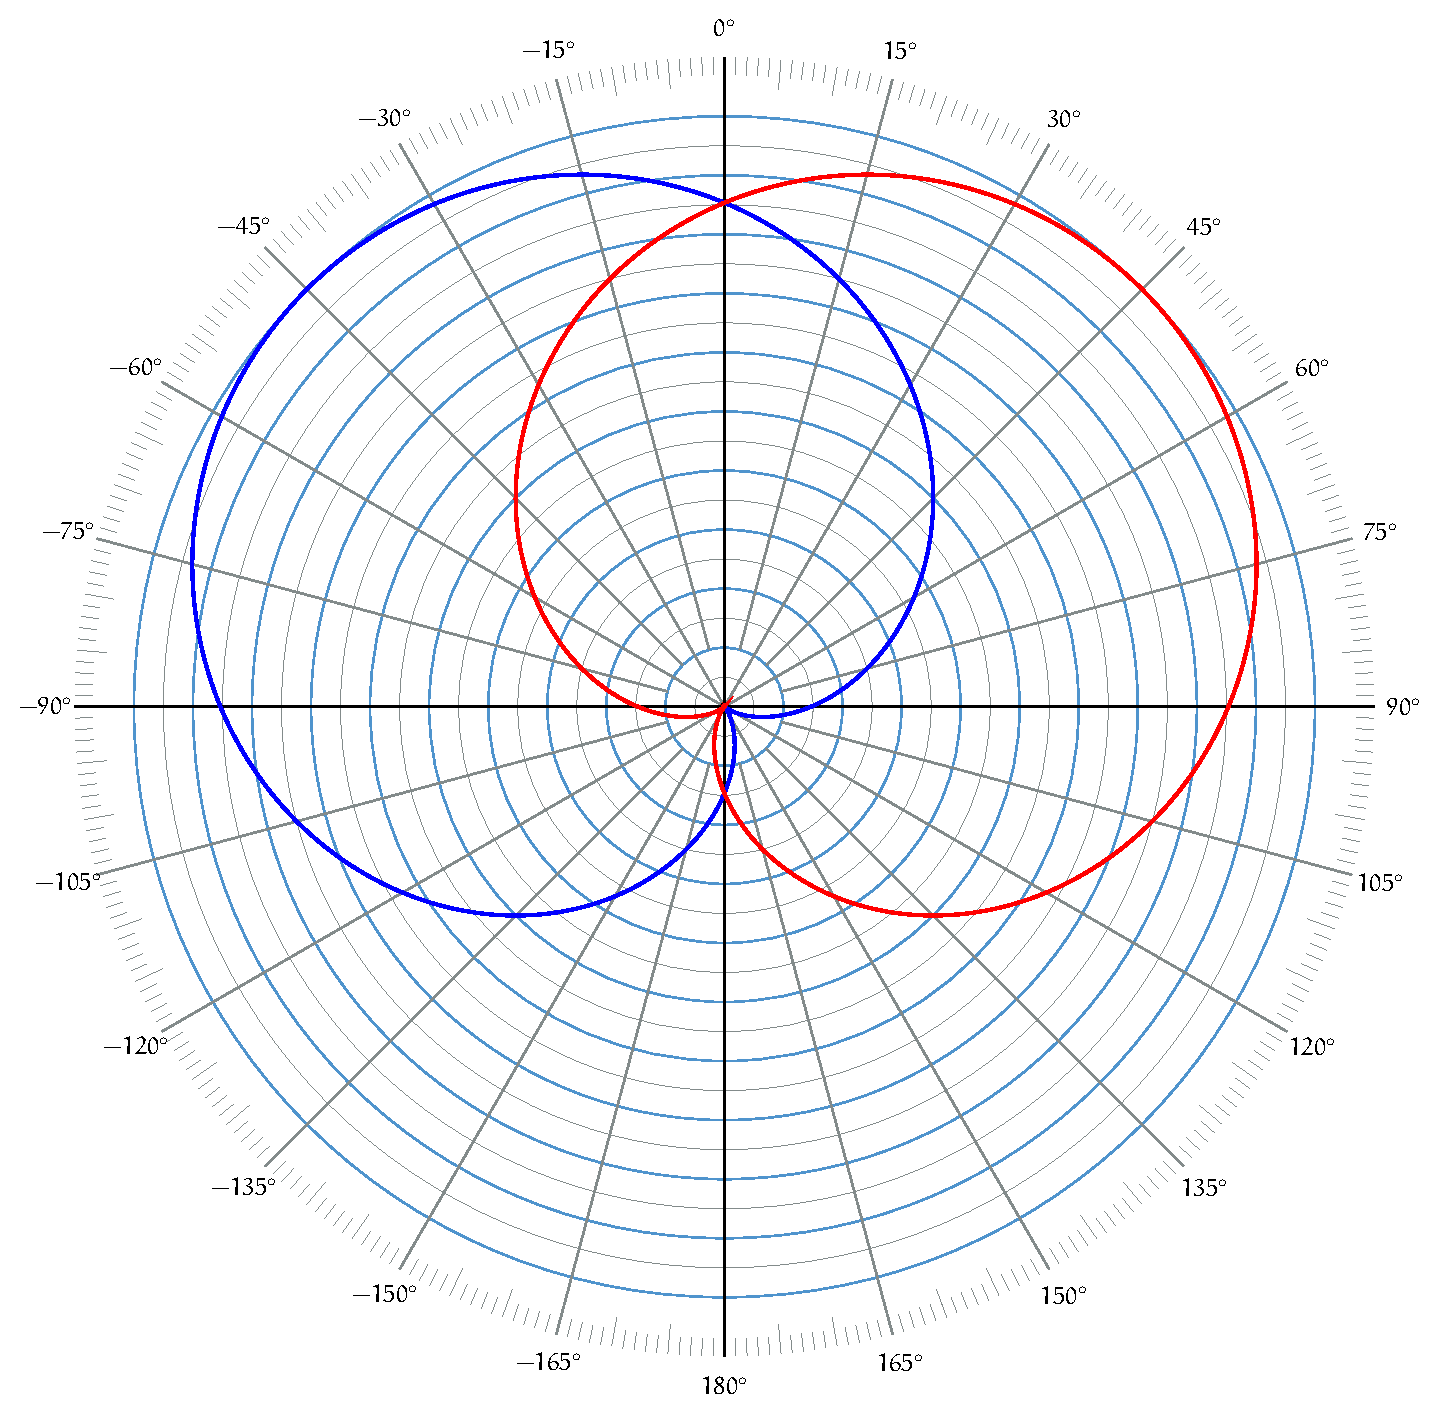
\includegraphics[height=6cm]{microphone-polar-patterns/xy90}
        \caption{Coppia stereofonica coincidente di cardioidi angolati di 90 gradi tra loro in entrata alla matrice.}% \\ Eq: $1(x)$}
        \label{pol:xy90ms}
    \end{subfigure}%
    ~
    \begin{subfigure}[t]{0.48\textwidth}
        \centering
        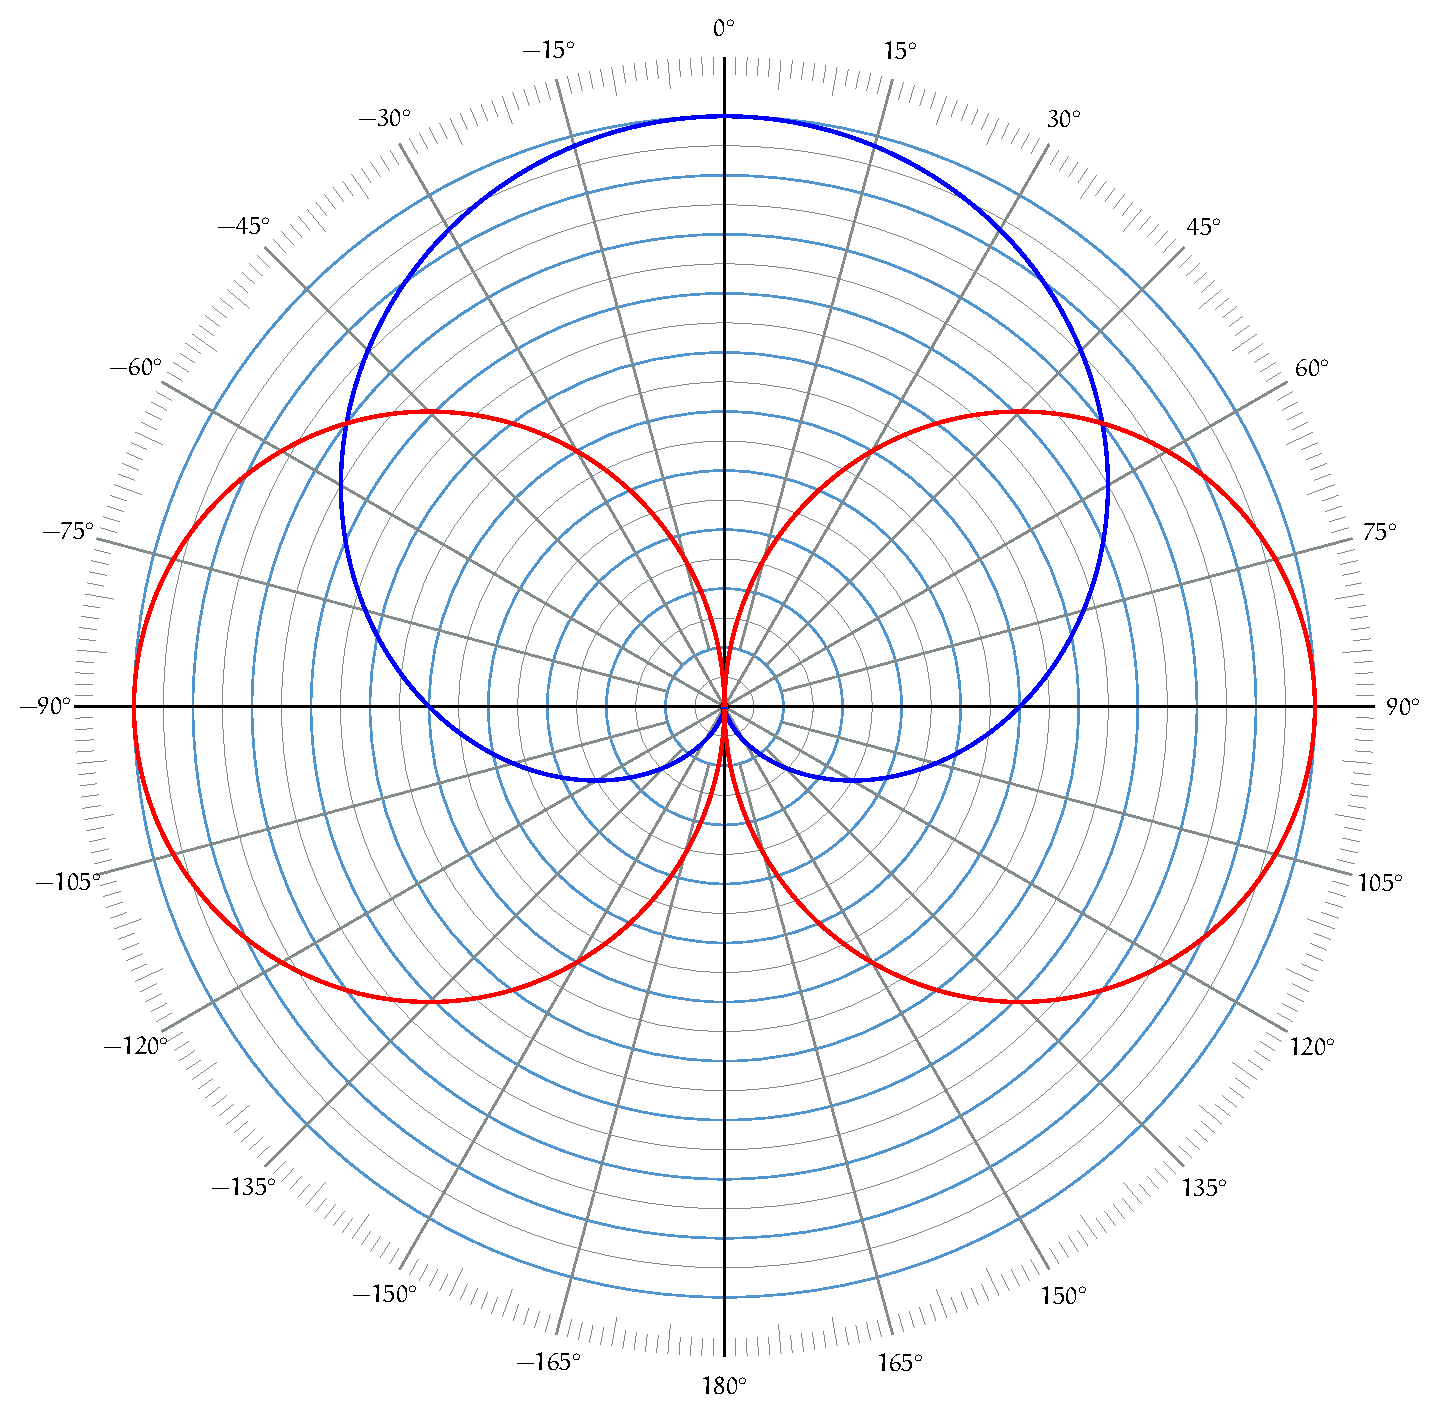
\includegraphics[height=6cm]{microphone-polar-patterns/midside}
        \caption{Le componenti \emph{Mid-Side} in uscita.}% \\ Eq: $0.75(x)+0.25(x\cos\theta)$}
        \label{pol:midsidems}
    \end{subfigure}
    \caption{Rappresentazione polare ideale del transito di una coppia \emph{xy90}
    attraverso la matrice e relativa rappresentazione d'uscita \emph{Mid-Side}.}
    \label{pol:msmatrix}
\end{figure*}

La matrice di Blumlein di somma e differenza tra i segnali è bidirezionale.
Quando il canale sinistro e destro di una coppia stereofonica passa attraverso la
matrice, la somma di entrambi i canali fornisce il segnale \emph{Mid} contenente solo le componenti in fase,
mentre la differenza produce il segnale \emph{Side} laterale contenente solo
componenti non in fase tra loro. Quando sono le componenti \emph{Mid-Side} a transitare
attraverso la matrice, la somma di \emph{Mid} e \emph{Side} fornisce la
correlazione tra fase sinistra e ampiezza, mentre la differenza produce la
correlazione tra fase negativa a ampiezza.

Di seguito il codice \emph{Faust} per la matrice somma e differenza.

%--------------------------------------------
%----------------larghezza massima del codice
\begin{lstlisting}
nsum = 0.5*(_+_);
ndif = 0.5*(_-_);
sdmx = _,_ <: nsum, ndif;
\end{lstlisting}

\begin{figure}[ht]
  \centering
  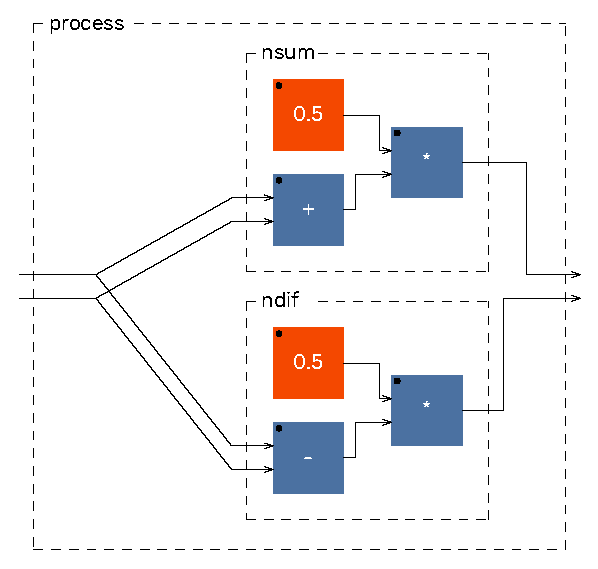
\includegraphics[]{CAPITOLI/1000/IMG/sdmx}
  \caption{Matrice somma e sottrazione.}
  \label{bd:sdmx}
\end{figure}

%%%%%%%%%%%%%%%%%%%%%%%%%%%%%%%%%%%%%%%%%%%%%%%%%%%%%%%%%%%%%%%%%%%% SECTION SIX
%%%%%%%%%%%%%%%%%%%%%%%%%%%%%%%%%%%%%%%%%%%%%%%%%%%%%%%%%%%%%%%%%%%%%%%%%%%%%%%%
\subsection{Mid-Side \emph{mic}}
\label{subsec:msmic}

\begin{figure}[b!]
\centering
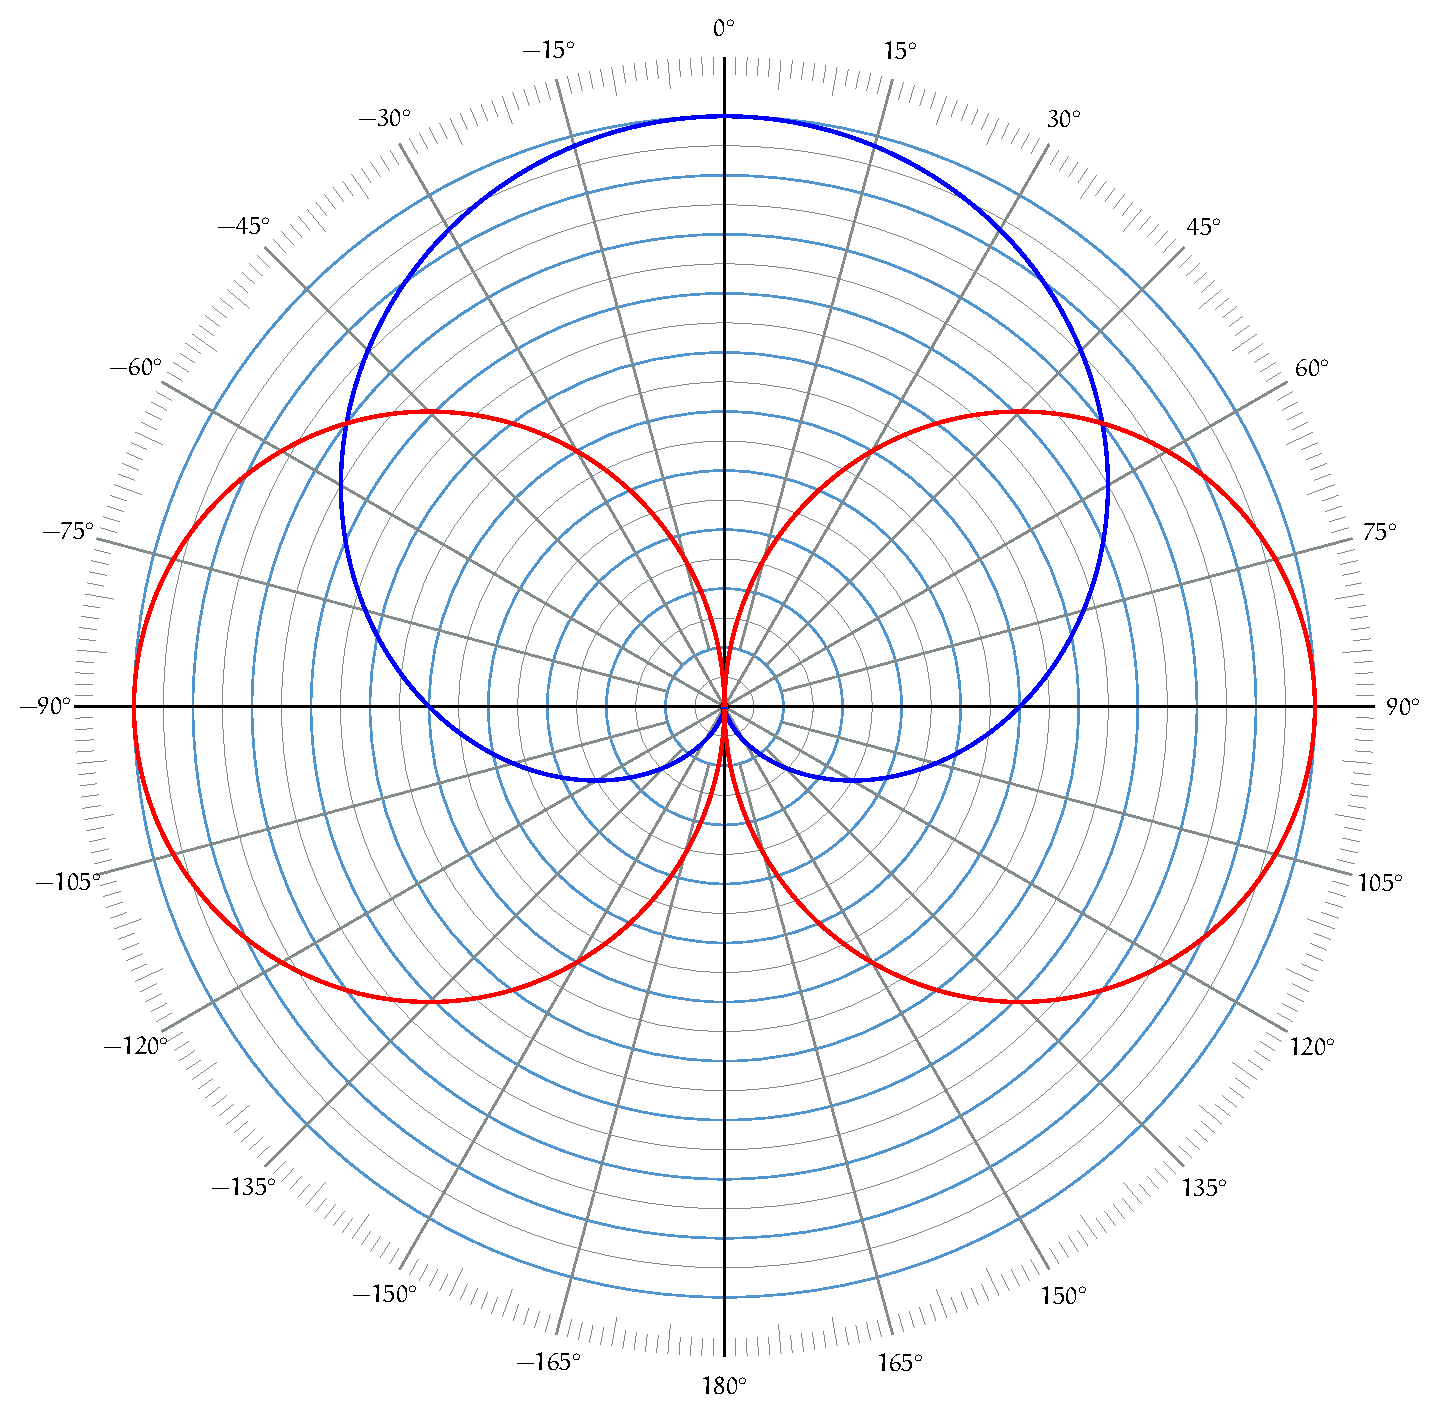
\includegraphics[width=0.99\columnwidth]{microphone-polar-patterns/midside}
\caption{Rappresentazione ideale della coppia stereofonica Mid-Side costituita da
da un microfono direzionale cardioide a gradiente di pressione mediante la sua
equazione polare: $cpg = 0.5(x) + 0.5(x\cos\theta)$ (\emph{cardioid pressure
gradient}) e da un microfono bidirezionale a gradiente di
pressione mediante la sua equazione polare: $bpg = x\cos\theta$
(\emph{bidirectional pressure gradient}). Nella tecnica microfonica di registrazione
Mid-Side il microfono cardioide convenzionalmente viene registrato nel primo canale,
mentre il segnale del microfono bidirezinale viene registrato nel secondo canale.}
\label{polar:midsidemic}
\end{figure}

La produzione di un segnale \emph{Mid-Side} come quello in uscita dalla matrice
somma e sottrazione può essere ottenuta dal posizionamento diretto di una coppia
di microfoni aventi caratteristiche polari adeguate. Il segnale \emph{Mid} è
generalmente prodotto da un microfono direzionale cardioide puntato verso il fronte
stereofonico, mentre il segnale \emph{Side} è generato da un microfono
bidirezionale puntato lateralmente, offrendo al fronte il punto di massimo
annullamento. I due microfoni devono essere allineati verticalmente in modo da
risultare orizzontalmente coincidenti.


%%%%%%%%%%%%%%%%%%%%%%%%%%%%%%%%%%%%%%%%%%%%%%%%%%%%%%%%%%%%%%%%%%%% SECTION SIX
%%%%%%%%%%%%%%%%%%%%%%%%%%%%%%%%%%%%%%%%%%%%%%%%%%%%%%%%%%%%%%%%%%%%%%%%%%%%%%%%
\subsection{Mid-Side \emph{panner}}
\label{subsec:mspanner}

La coppia stereofonica di segnali \emph{Mid-Side} è stata descritta finora come
risultante della matrice somma e sottrazione applicata ad un segnale stereofonico
oppure come segnale prodotto da una coppia di microfoni aventi caratteristiche
oppurtune. Analizziamo ora un terzo sistema in grado di generare una coppia
\emph{Mid-Side} attraverso un sistema di panning.

Il canale frontale \emph{Mid} è comunemente descritto da un microfono cardioide.
Sappiamo che la componente cardioide, come moltre altre figure polari, può
essere risultante da una combinazine misurata di
componenti non-direzionale e bidirezionale.

\begin{equation}
m(x,p,\theta) = (p*x) + ((1-p)*(x\cos\theta)
\label{eq:mid}
\end{equation}

Dove $x$ è il segnale di ingresso, $p$ è il coefficiente di ampiezza che regola
il rapporto di peso tra le due componenti, $0.5$ per ottenere la figura polare
cardioide, $\theta$ è la direzione di impatto angolare espressa in radianti.

La componente \emph{Side} è costituita dalla sola componente bidirezionale.

\begin{equation}
s(x,\theta) = x*(sin(\theta))
\label{eq:side}
\end{equation}

Il codice \emph{Faust} per la costruzione di un \emph{Mid-Side Panner} è
molto simile alle equazioni che descrivono le due figure polari.

%--------------------------------------------
%----------------larghezza massima del codice
\begin{lstlisting}
mspan(x,p,rad) = m,s
with{
  m = (p*x)+((1-p)*(x*cos(rad)));
  s = x*(sin(-rad));
};
\end{lstlisting}

I due segnali in uscita dal panner non possono essere inviati direttamente ad un
sistema di ascolto basato sui due canali sinistra-destra, devono necessariamente
passarli attraverso la matrice somma e differenza ottenere ciò che Blumlein
descrive come la differenza di ampiezza nei segnali degli altoparlanti
ottenuta dalle differenze di fase.

% %--------------------------------------------
% %----------------larghezza massima del codice
% \begin{lstlisting}
% mspan_lr(x,p,rad) = mspan(x,p,rad) : sdmx;
% \end{lstlisting}

\begin{figure}[t]
\centering
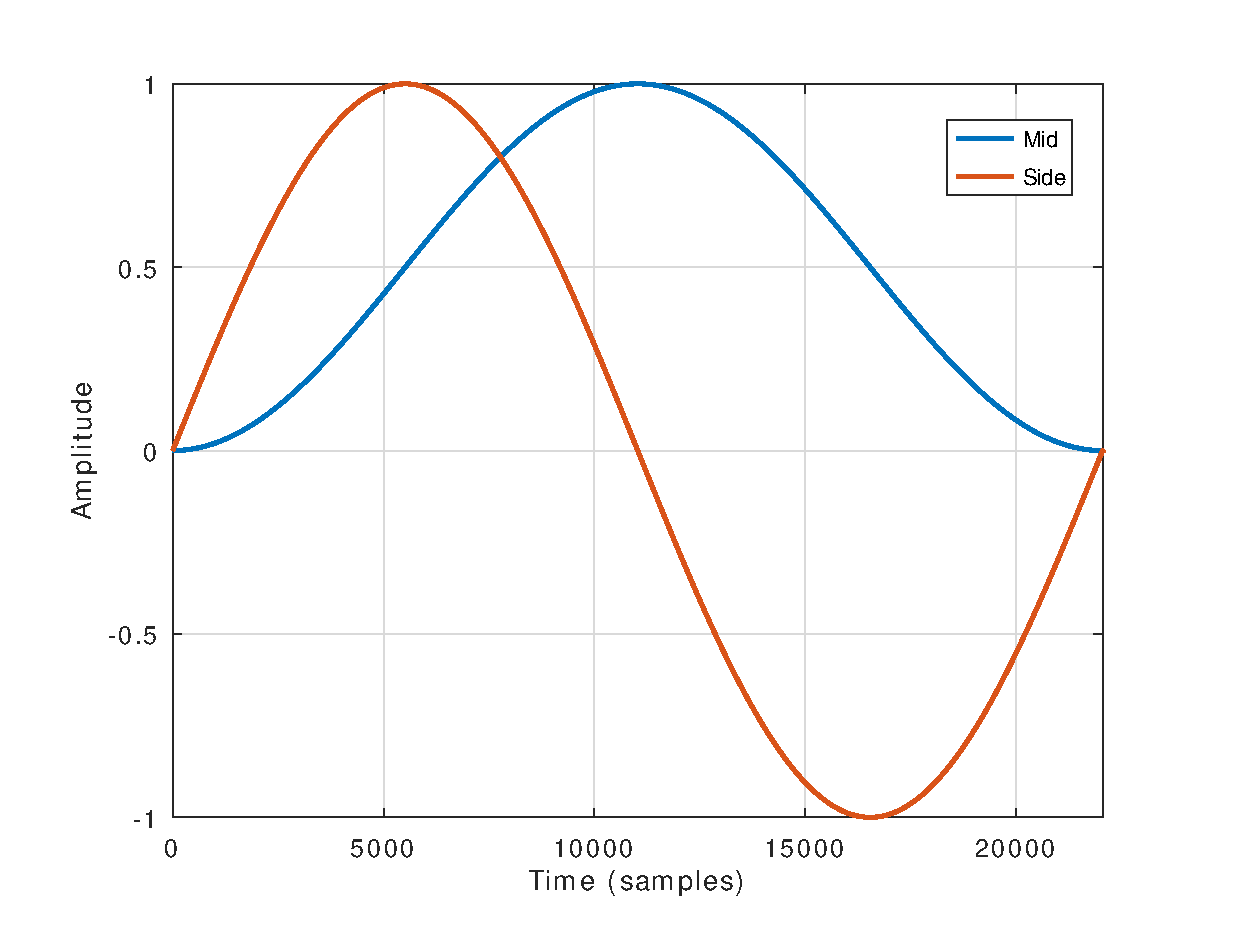
\includegraphics[width=0.99\columnwidth]{CAPITOLI/1000/IMG/mspan}
\caption{Mid-Side \emph{panner}. Il grafico mostra la risposta del \emph{panner} ad una
variazione di 360 gradi da sinistra (-180 gradi) a destra (180 gradi). La linea
rossa mostra la bipolarità del segnale correlata alle informazioni angolari. La
linea blu descrive variazioni di ampiezza (sempre con fase positiva) in
relazione alle informazioni angolari. Il grafico mostra l'evidenza della percezione
zero su entrambi gli estremi $\pm180$ gradi, dove cardioide e figura-8 si annullano.}
\label{fig:mspan}
\end{figure}

% La procedura di costruzione dell'algoritmo del \emph{Mid-Side Panner} è completa.
% Il seguente codice di \emph{Faust} descrivo il panner completo di interfaccia
% grafica.

%-----------------------------------------------------------
%-------------------------------larghezza massima del codice
\begin{lstlisting}
//----------------------------------- DEGREES TO RADIANS ---
deg2rad = *(ma.PI/180);
//----------------------------------------------- PANPOT ---
rad = vslider("[02]Azimuth[style:knob]", 0,-180,180,0.1) :
      deg2rad : si.smoo;
//--------------------------------------------- P FACTOR --–
p = vslider("[01]P[style:knob]", 0.5,0,1,0.01) : si.smoo;
//--------------------------------------------- MID-SIDE --–
midside(x,p,rad) = m,s
  with{
    m = (p*x)+((1-p)*(x*cos(rad)));
    s = x*(sin(-rad));
};
//-------------------------------- MS MATRIX DESCRIPTION ---
nsum = 0.5*(_+_);
ndif = 0.5*(_-_);
sdmx = _,_ <: nsum, ndif;
//----------------------------------------- MS2LR MATRIX ---
mspan_lr(x,p,rad) = midside(x,p,rad) : sdmx;
process = os.osc(1000), p, rad : mspan_lr;
\end{lstlisting}

